\chapter[Analyse du sujet]{Analyse du sujet}

\textit{Une phase d'analyse du sujet a été préalablement réalisée. Ce premier chapitre a pour objectif de rappeler les éléments de contexte et la problématique du sujet. Il rappellera également les fonctionnalités initialement prévues dans le programme.}

\section{Définition du sujet}

\subsection{Contexte}

Le projet s’inscrit dans le cadre des recherches du laboratoire MATIS de l'IGN pour la reconstruction 3D des bâtiments à partir de Modèles Numériques de Surface (MNS). Pour détecter et caractériser les erreurs de reconstruction, l’équipe de recherche a mis en place une méthode d’auto-qualification. Ce processus passe par la réalisation d’une classification supervisée des entités reconstruites, afin de leur associer une classe d’erreur.

\subsection{Problématique et analyse des besoins}

L’objectif est d’évoluer vers une classification active. En effet, l’intervention d’un utilisateur permettrait de valider les résultats de la classification, afin d’affiner le modèle de prédiction entrainé.\\

Le projet de programmation présenté dans ce rapport est donc un outil graphique d'aide à la classification active. Grâce à une interface, l'utilisateur peut visualiser certains objets d'intérêt (orthophoto et bâtiments orthoprojetés) . Il peut ensuite valider le résultat de la classification, ou dans le cas contraire de renseigner la bonne erreur.\\

\begin{figure}[!h]
	\begin{center}
		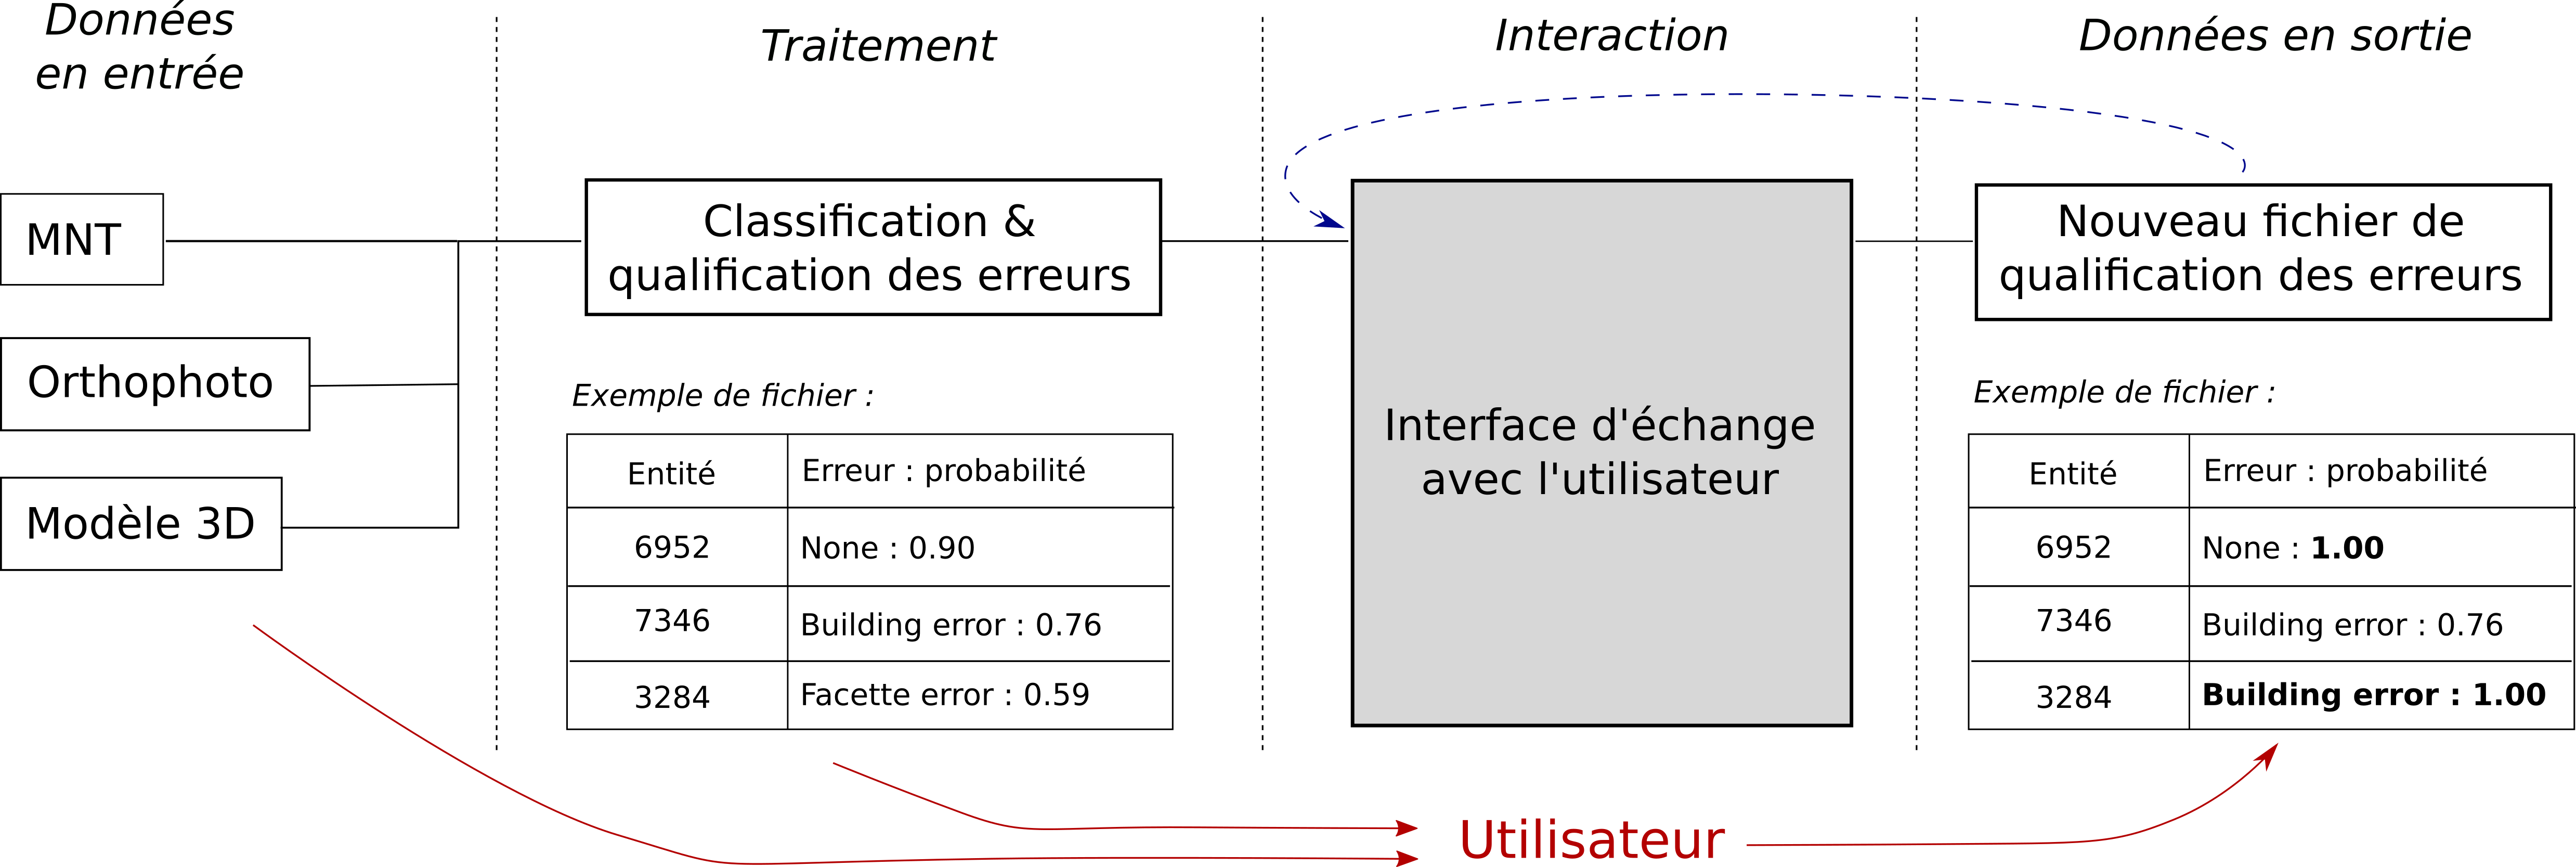
\includegraphics[scale=0.35]{Process_projet.png}  \\
		\caption[Chaîne de traitement simplifiée du projet]{Chaîne de traitement simplifiée du projet}
		\label{fig:processprojet}
	\end{center}
\end{figure}

\textit{Cette section a permis de retracer les principaux objectifs du projet. Le développement suivant vise à détailler les principales fonctionnalités envisagées lors de l'analyse.}

\section{Analyse fonctionnelle}

\subsection{Organisation des données}

Le programme considère plusieurs données en entrée, sélectionnées par l'utilisateur via une première interface :

\renewcommand{\arraystretch}{1.4}
\begin{figure}[!h]
	\begin{center}
		\begin{tabular}{|c|c|c|}
			\hline
			Données & Type de donnés & Correspondance dans le code \\
			\hline
			Classes d'erreurs possibles & Fichier .CSV & Variable de type dictionnaire \\
			Résultats de l'auto-qualification & Fichier .CSV & Liste de tuples \\
			Géométrie des entités & Dossier de .SHP & Attribut \textit{geometry} de la classe Bâtiment\\
			Orthophoto & Fichier .TIFF & Tuple (résolution + référence) + Matrice\\
			\hline
		\end{tabular}
	\end{center}
	\caption[Données en entrée]{Données en entrée}
	\label{tab:dataentre}
\end{figure}

\noindent De même, le formalisme des données en sortie est imposé :

\renewcommand{\arraystretch}{1.4}
\begin{figure}[!h]
	\begin{center}
		\begin{tabular}{|c|c|c|}
			\hline
			Données & Type de donnés & Correspondance dans le code \\
			\hline
			Résultats de l'interaction & Fichier .CSV & Liste de tuples \\
			\hline
		\end{tabular}
	\end{center}
	\caption[Données en sortie]{Données en sortie}
	\label{tab:datasortie}
\end{figure}

\subsection{Principales fonctionnalités}

\begin{figure}[!h]
	\begin{minipage}{0.50\linewidth}\parindent12pt
		 \indent L'interface doit permettre à un utilisateur de visualiser et de contrôler les résultats d'une classification. Ainsi, les principales fonctionnalités à développer sont :\\
		\begin{itemize}[label=$\rightarrow$]
			\item Une interface de chargement des données ;
			\item Une fonction de sélection des entités à présenter à l'utilisateur ;
			\item Une interface de visualisation graphique et textuelle des entités ;
			\item Une fonction de contrôle des entités par l'utilisateur.
		\end{itemize}
	\end{minipage}
\hfill
	\begin{minipage}{0.45\linewidth}
		\centering
		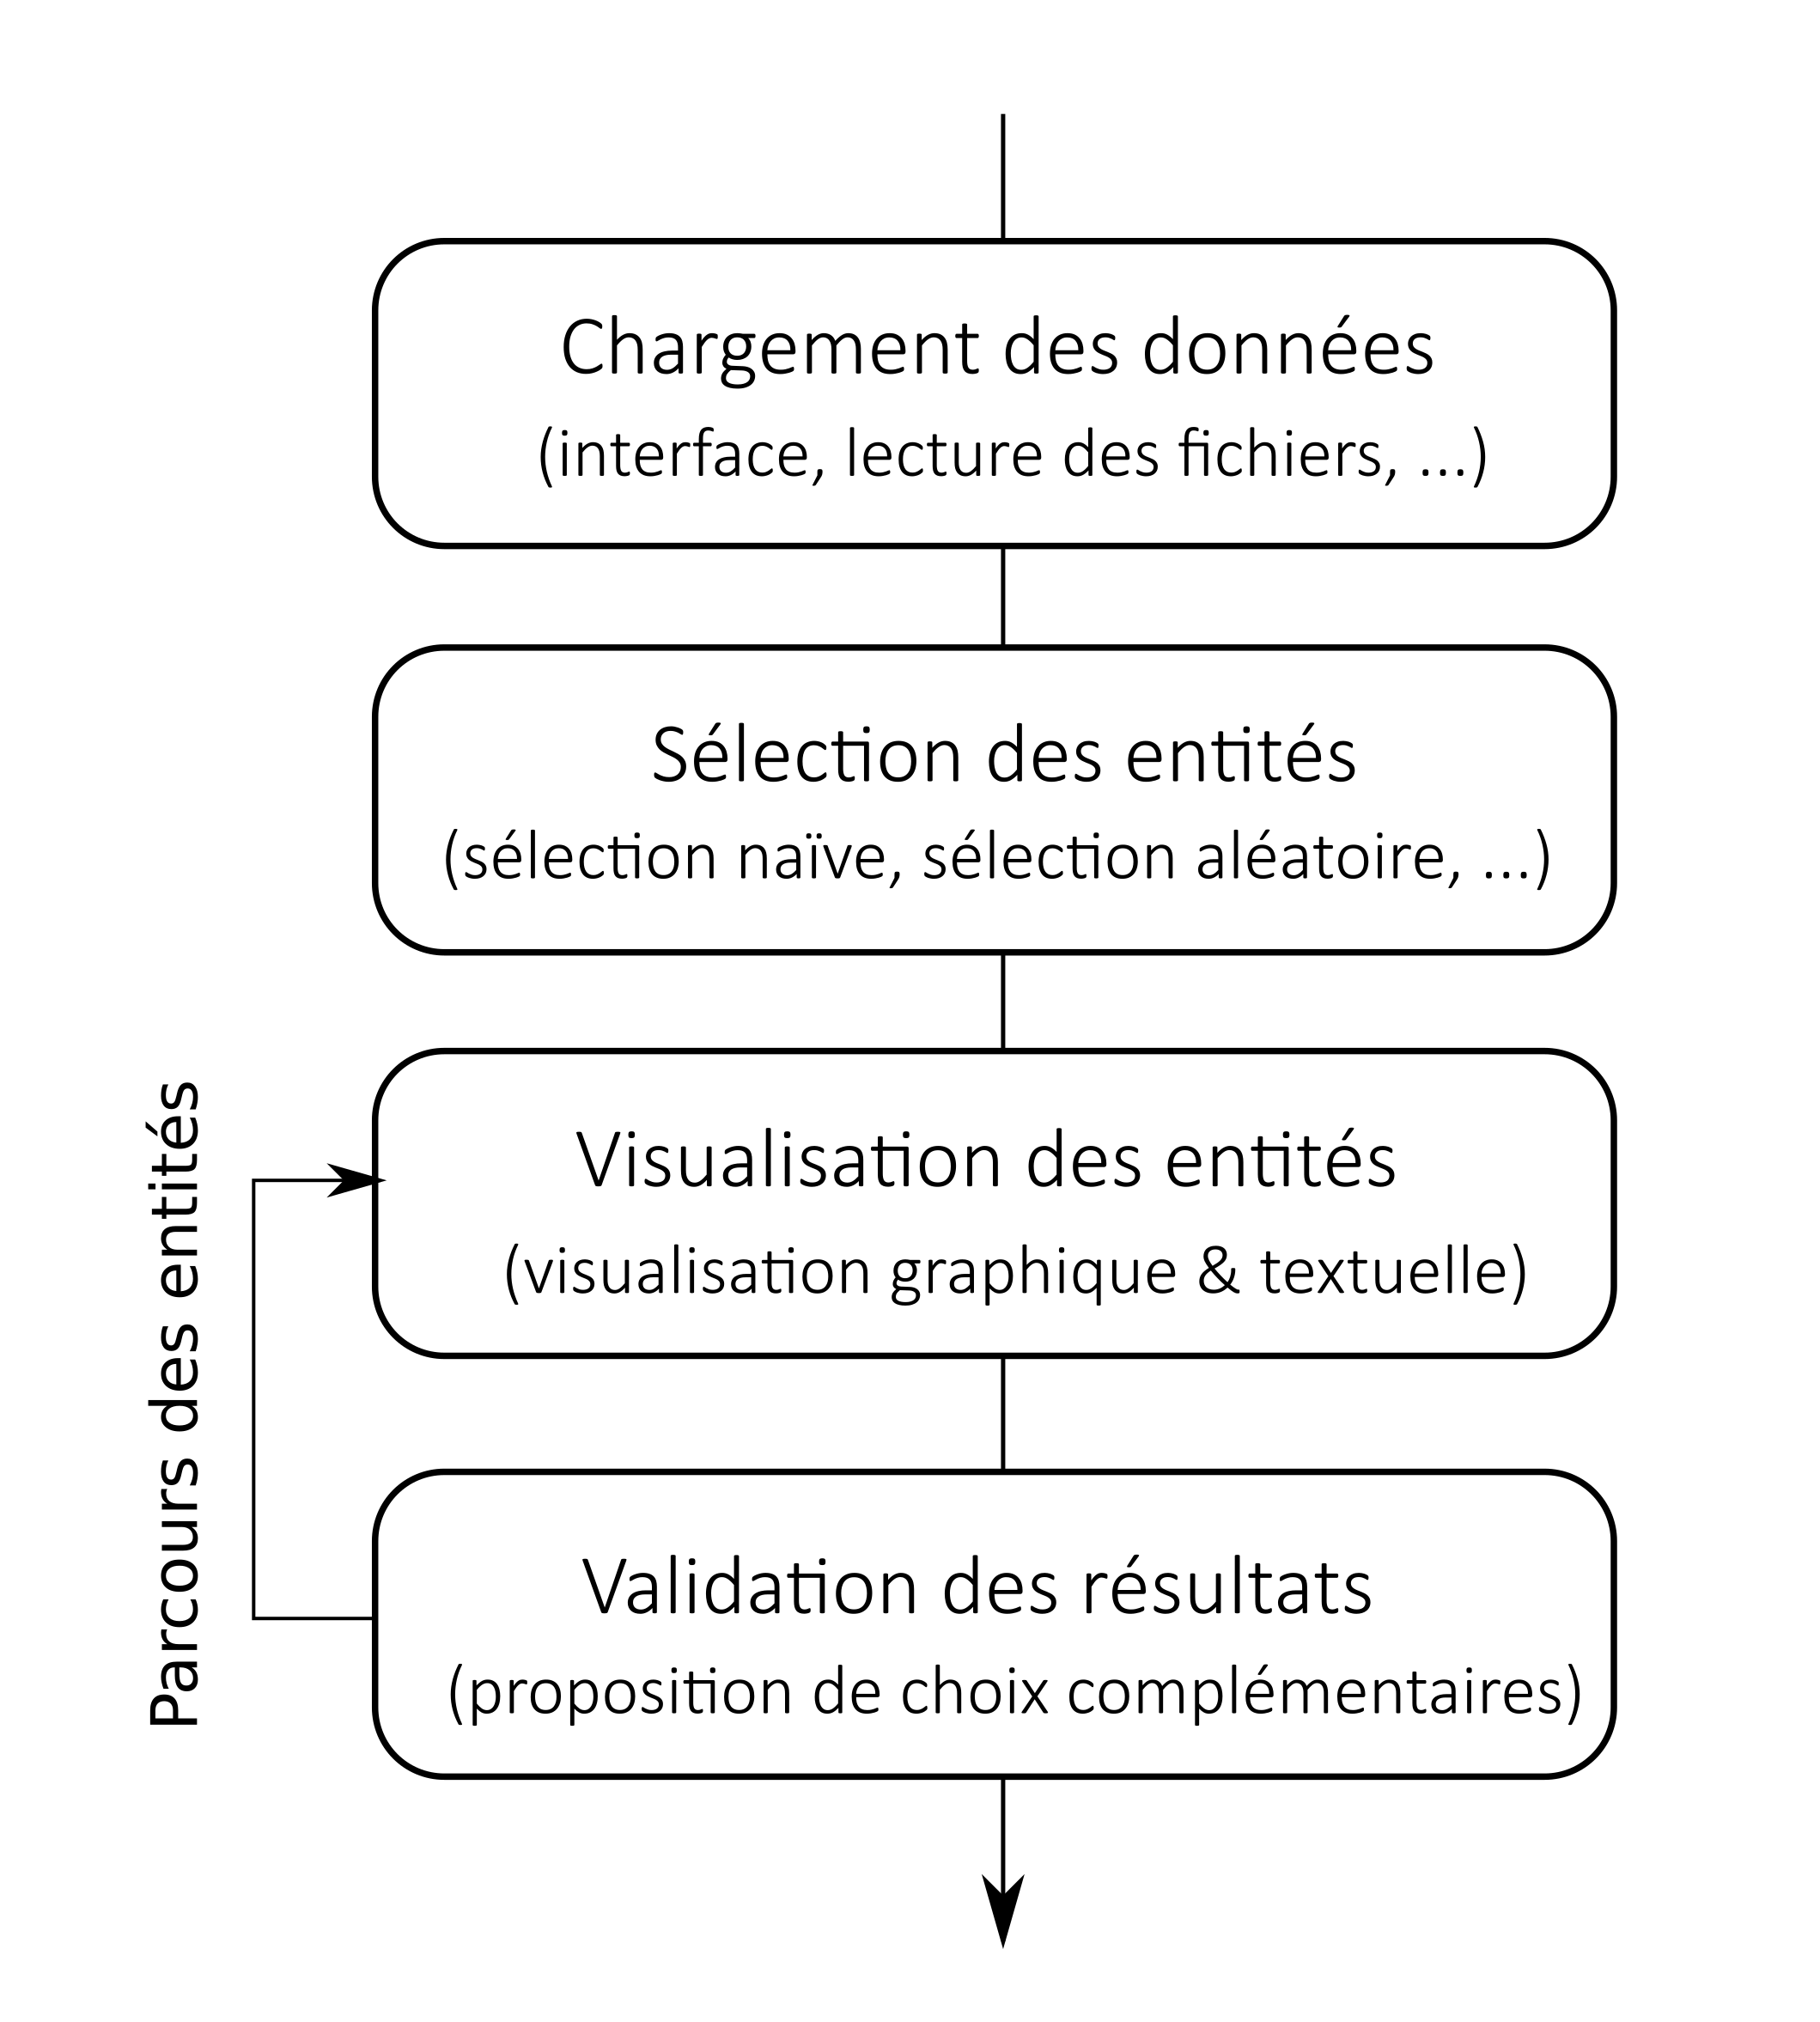
\includegraphics[scale=0.30]{Fonctionnalites_principales.png}  \\
		\caption[Fonctionnalités principales]{Fonctionnalités principales}
		\label{fig:fonctionnalitesprinc}
	\end{minipage}
\end{figure}

\textit{Après avoir rappelé les principales fonctionnalités du programme et les données nécessaires à son fonctionnement, on rappellera les choix techniques réalisés.}

\section{Choix techniques}

L’interface graphique voulue pour ce projet utilise la bibliothèque Qt associée à un script Python (PyQt5). Cela lui permet de fonctionner sur tous les environnements informatiques, et elle peut être modulée sans prendre en compte le formalisme de QGIS.
